% Provenance (never printed): see sources/outline_sources.md (Year 1: field
% notebook, compass-clinometer, hand lens, sampling, polarising microscope and
% thin sections, safety). The readings of the Varden east limb are simulated
% in figdata/bachelor-1/attitude_stats.py (seed 83, errors of 3 degrees);
% problem values in the Book 3 scratch calculator calc/ch06.py.
\chapter{Méthodes de terrain et de laboratoire I}\label{ch:b1:field-lab-methods-1}

Une géologue qui cartographie les collines de Varden emporte peu de choses~: un
carnet, un crayon, un récepteur satellitaire, une boussole à clinomètre, une
loupe et quelques sacs d'échantillons. Avec eux, elle fixe l'endroit où elle se
trouve, mesure l'\omterm{def:b1:geological-maps:attitude}{attitude} des couches, nomme les roches, et rapporte les
échantillons que le laboratoire coupera, polira et regardera au microscope.
Chaque nombre des chapitres précédents --- une \omterm{def:b1:geological-maps:attitude}{attitude} sur une carte, un
\omterm{def:b1:geological-maps:attitude}{pendage} sur une coupe --- a commencé comme une lecture de ce genre, avec son
erreur propre. Ce chapitre décrit comment les professionnels font ces
observations, et comment on moyenne des lectures répétées et on transforme leur
dispersion en incertitude. Il se termine par une saison de lectures sur le flanc
est de l'\omterm{def:b1:geological-maps:fold}{anticlinal} de Varden.

\begin{recall}
L'\omterm{def:b1:geological-maps:attitude}{attitude} d'un plan s'écrit \omterm{def:b1:geological-maps:attitude}{sens du pendage}/\omterm{def:b1:geological-maps:attitude}{pendage}, comme $081/12$, ou bien par
une direction obtenue par la règle de la main droite avec un \omterm{def:b1:geological-maps:attitude}{pendage}
(\cref{ch:b1:geological-maps}). La déclinaison magnétique est l'angle entre le
nord géographique et la direction vers laquelle pointe l'aiguille d'une boussole
(physique, année~11). Les minéraux se reconnaissent à la main par leur éclat,
leur clivage, leur dureté et leur couleur (livre~2, année~11). La moyenne et
l'écart type d'un ensemble de nombres résument leur centre et leur dispersion
(mathématiques).
\end{recall}

\section{Le carnet et la carte}

\begin{definition}[Station d'observation, carnet de terrain]\label{def:b1:field-lab-methods-1:station}
Une \emph{station d'observation}\index{station d'observation} est un lieu numéroté où un géologue fait et consigne des
observations~: sa position, les roches vues, leur \omterm{def:b1:geological-maps:attitude}{attitude}, et les échantillons
prélevés. Le \emph{carnet de terrain}\index{carnet de terrain} est le registre relié des stations, dans
l'ordre où elles ont été visitées, avec leurs numéros, croquis et mesures,
écrit sur place.
\end{definition}

Le carnet est l'enregistrement primaire~: ce qui n'est pas écrit à la station est
perdu, et une carte dessinée le soir ne vaut que les notes qui la sous-tendent.
Chaque station a un numéro qui figure sur la carte de terrain, dans le carnet et
sur chaque sac d'échantillon prélevé là. Un croquis montre ce qu'une liste de
nombres ne peut pas montrer --- comment deux unités se rencontrent, de quel côté
se trouvent les couches les plus jeunes, où une lecture a été prise sur une
surface plissée --- et note son échelle et son orientation. Les faits et les
interprétations sont tenus séparés~: «~calcaire sur argilite, contact net~» est
une observation~; «~\omterm{def:b1:cross-sections:unconformity}{discordance}~» est une inférence, écrite comme telle.

\begin{inthefield}[Une journée de cartographie]
% ledger: gps:smartphone-accuracy, gps:high-end
\begin{minipage}[t]{0.58\linewidth}\vspace{0pt}
Une géologue cartographe prévoit un itinéraire en travers de la direction des
couches, de façon à rencontrer chaque unité tour à tour, et s'arrête partout où
apparaît un contact, un changement de roche ou une surface mesurable. À chaque
station, elle note le numéro de la station et la position, croque ce qu'elle
voit, mesure des \omterm{def:b1:geological-maps:attitude}{attitudes} et note les échantillons. Les positions viennent d'un
récepteur satellitaire~: un récepteur ordinaire, comme celui d'un téléphone
intelligent, est typiquement précis à environ \qty{4.9}{m} sous ciel dégagé,
moins près des falaises et des arbres, tandis que les récepteurs de géomètre
utilisant deux fréquences ou des services de correction atteignent quelques
centimètres. À l'échelle de 1:10\,000, \qty{4.9}{m} valent un demi-millimètre~:
un récepteur ordinaire suffit pour cartographier, mais pas pour mesurer le lent
mouvement du sol (\cref{ch:b1:plate-kinematics}).
\end{minipage}\hfill
\begin{minipage}[t]{0.39\linewidth}\vspace{0pt}
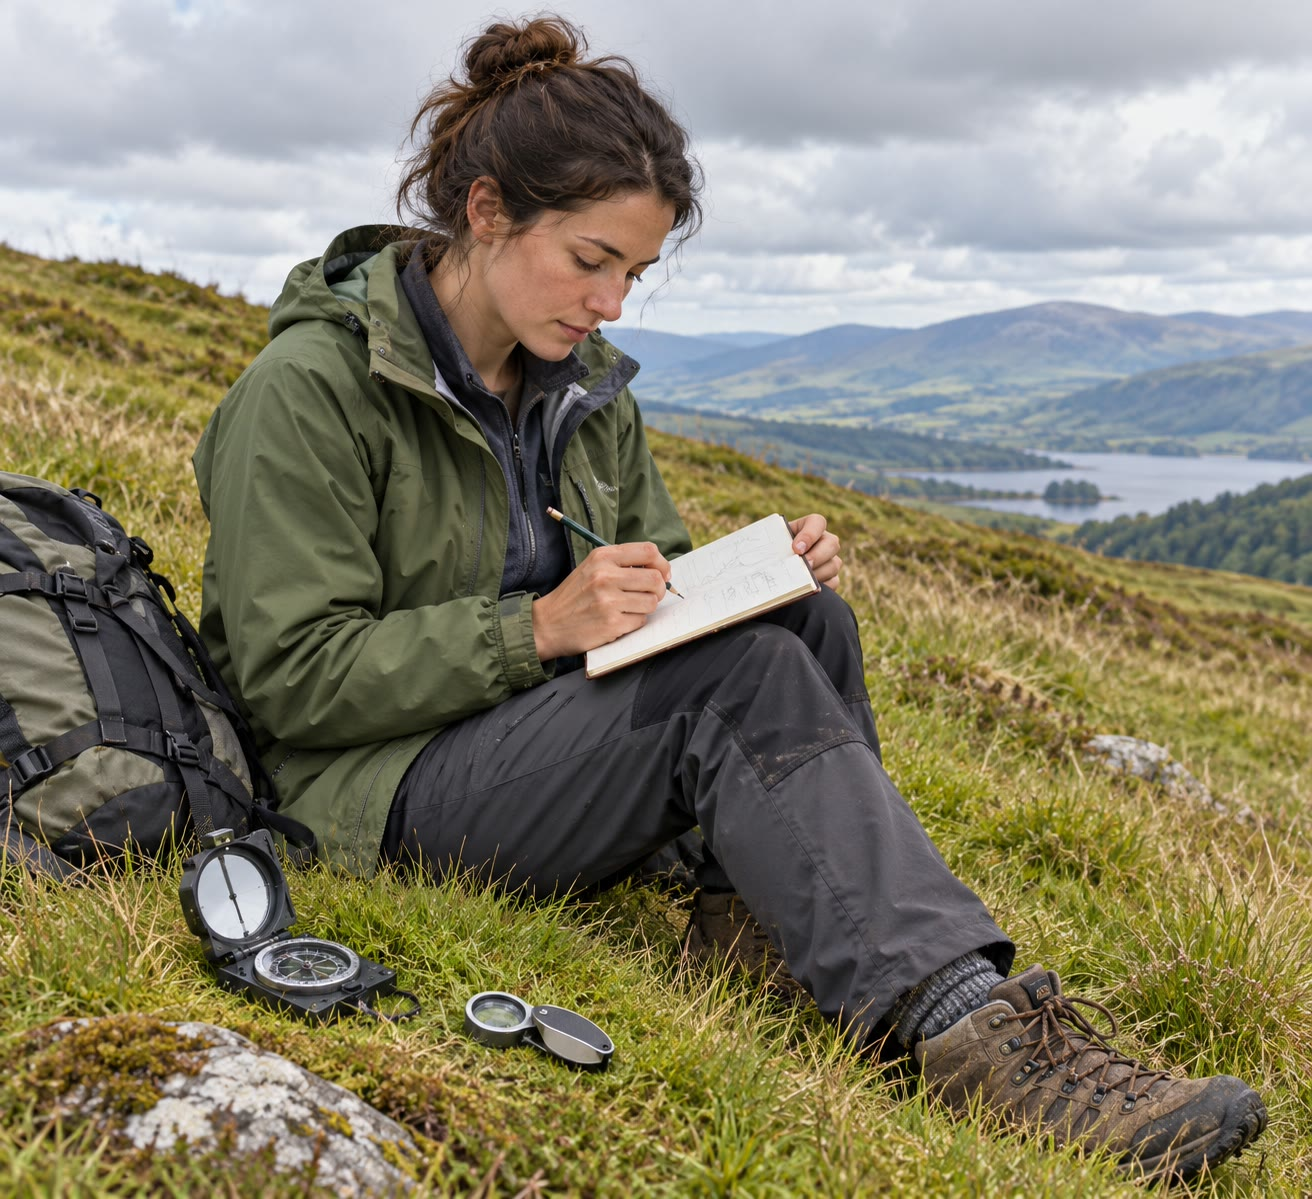
\includegraphics[width=\linewidth]{images/book3/ai/b1-field-notebook.jpg}
\end{minipage}
\end{inthefield}

\section{Mesurer des orientations}

L'\omterm{def:b1:geological-maps:attitude}{attitude} d'un plan --- une couche, une faille, un joint --- se mesure avec une
boussole à clinomètre~: une boussole magnétique pour lire les \omterm{def:b1:spherical-astronomy:horizontal}{azimuts}, et un
pendule ou un niveau pour lire les angles à partir de l'horizontale. On pose son
bord le long de la direction de la surface pour lire la direction, ou l'on place
l'instrument sur la surface le long de sa ligne de plus grande pente pour lire le
\omterm{def:b1:geological-maps:attitude}{pendage} et, d'après l'\omterm{def:b1:spherical-astronomy:horizontal}{azimut} de cette ligne, le \omterm{def:b1:geological-maps:attitude}{sens du pendage}.

\begin{omfigure}
\begin{tikzpicture}[font=\scriptsize]
% (a) plan view
\begin{scope}
\fill[icsJurassic!25] (0,0) -- (3.6,0.5) -- (3.9,2.9) -- (0.3,2.4) -- cycle;
\draw (0,0) -- (3.6,0.5) -- (3.9,2.9) -- (0.3,2.4) -- cycle;
\draw[omDef, thick] (0.4,1.55) -- (3.5,1.98);
\node[omDef, above, rotate=8, fill=icsJurassic!25, inner sep=1pt] at (0.95,1.65) {direction};
% compass box laid along the strike line
\begin{scope}[shift={(2.5,1.84)}, rotate=8]
\draw[fill=white] (-0.6,0) rectangle (0.6,0.32);
\draw (0,0.16) circle (0.12);
\end{scope}
\draw[omThm, thick, -{Stealth[length=2mm]}] (1.6,1.71) -- (1.75,0.62);
\node[omThm, right, fill=icsJurassic!25, inner sep=1pt] at (1.78,0.85) {sens du pendage};
\node[below, align=center] at (1.95,-0.15) {(a) vue en plan~: bord de la\\ boussole le long de la direction};
\draw[->] (4.3,1.6) -- (4.3,2.4) node[above] {N};
\end{scope}
% (b) side view, vertical section along the dip direction
\begin{scope}[xshift=5.8cm]
\fill[icsJurassic!25] (0,1.6) -- (3.6,0.2) -- (3.6,-0.3) -- (0,-0.3) -- cycle;
\draw[thick] (0,1.6) -- (3.6,0.2);
% clinometer resting on the surface
\begin{scope}[shift={(2.5,0.6278)}, rotate=-21.25]
\draw[fill=white] (-0.75,0) rectangle (0.75,0.3);
\draw (0,0.15) circle (0.11);
\draw[black!70] (0,0.15) -- ++(-68.75:0.11);
\end{scope}
% dip angle at the lower end of the surface
\coordinate (P) at (0.7,1.3278);
\draw[black!60] (P) -- ++(1.6,0) node[right] {horizontale};
\draw[omThm] ($(P)+(1.1,0)$) arc[start angle=0, end angle=-21.25, radius=1.1];
\node[omThm] at ($(P)+(0.9,-0.15)$) {$\delta$};
\node[below, align=center] at (1.8,-0.35) {(b) coupe selon le pendage~:\\ clinomètre sur la plus grande pente};
\end{scope}
\end{tikzpicture}

{\small Mesure d'une \omterm{def:b1:geological-maps:attitude}{attitude} (schématique). (a) Le bord de la boussole posé
horizontalement sur la couche donne la direction~; le \omterm{def:b1:geological-maps:attitude}{sens du pendage} lui est
perpendiculaire, vers le bas de la couche. (b) Posé sur la tranche le long de la
ligne de plus grande pente, le clinomètre donne le \omterm{def:b1:geological-maps:attitude}{pendage} $\delta$.}
\end{omfigure}

Une ligne --- un axe de \omterm{def:b1:geological-maps:fold}{pli}, une strie sur une surface de faille, le grand axe de
galets --- a une orientation propre.

\begin{definition}[Direction et plongement d'une ligne]\label{def:b1:field-lab-methods-1:trend-plunge}
La \emph{direction d'une ligne}\index{direction (d'une ligne)} est l'\omterm{def:b1:spherical-astronomy:horizontal}{azimut} de sa
projection horizontale, mesuré vers l'extrémité de la ligne qui pointe vers le
bas. Son \emph{plongement}\index{plongement} est l'angle entre la ligne et
l'horizontale, mesuré dans le plan vertical qui la contient. Une ligne plongeant
de \ang{20} vers \ang{015} s'écrit $20\to015$.
\end{definition}

Une ligne d'\omterm{def:b1:spherical-astronomy:horizontal}{azimut} $t$ (sa direction) et de \omterm{def:b1:field-lab-methods-1:trend-plunge}{plongement} $p$ a pour vecteur
unitaire descendant
$(\cos p\sin t, \cos p\cos t, -\sin p)$ en composantes est, nord et haut~;
une ligne contenue dans un plan de \omterm{def:b1:geological-maps:attitude}{sens du pendage} $\alpha$ et de \omterm{def:b1:geological-maps:attitude}{pendage}
$\delta$ plonge du \omterm{def:b1:cross-sections:apparent-dip}{pendage apparent} de ce plan dans le plan vertical d'\omterm{def:b1:spherical-astronomy:horizontal}{azimut}
$t$, de sorte que
$\tan p = \tan\delta\cos(\alpha - t)$ (\cref{thm:b1:cross-sections:apparent-dip}).

\subsection{La déclinaison magnétique}

L'aiguille d'une boussole pointe vers le nord magnétique, non vers le nord
géographique~; l'angle entre les deux est la déclinaison magnétique, comptée
positivement quand le nord magnétique est à l'est du nord géographique. Les
cartes et les \omterm{def:b1:geological-maps:attitude}{attitudes} de ce livre utilisent des \omterm{def:b1:spherical-astronomy:horizontal}{azimuts} géographiques.

\begin{method}[Corriger l'azimut d'une boussole]\label{met:b1:field-lab-methods-1:declination}
\begin{enumerate}
  \item Trouver la déclinaison magnétique $D$ pour le lieu et la date, à partir
        d'un modèle du champ de la Terre (positive à l'est, négative à l'ouest).
  \item L'ajouter à chaque \omterm{def:b1:spherical-astronomy:horizontal}{azimut} lu sur la boussole~: \omterm{def:b1:spherical-astronomy:horizontal}{azimut} géographique $=$
        \omterm{def:b1:spherical-astronomy:horizontal}{azimut} magnétique $+ D$, pris modulo \ang{360}.
  \item Ne pas toucher aux \omterm{def:b1:geological-maps:attitude}{pendages} et aux \omterm{def:b1:field-lab-methods-1:trend-plunge}{plongements}~: ils se mesurent à partir
        de l'horizontale, avec la pesanteur, et non avec l'aiguille.
\end{enumerate}
La plupart des boussoles de terrain peuvent être réglées pour ajouter $D$
mécaniquement~; le réglage, et l'année pour laquelle il a été fait, sont notés
dans le carnet.
\end{method}

\begin{dated}{2026}
% ledger: noaa:wmm-edinburgh, noaa:wmm-reykjavik, noaa:wmm-anchorage, noaa:wmm-wellington
Au 1\textsuperscript{er} janvier 2026, le modèle magnétique mondial (version
2025) donne la déclinaison magnétique de \ang{-0.47} (ouest) à Édimbourg, avec
une variation de \ang{+0.20} par an~; \ang{-11.28} à Reykjavik, avec une
variation de \ang{+0.30} par an~; \ang{+14.20} (est) à Anchorage, avec une
variation de \ang{-0.28} par an~; et \ang{+23.23} à Wellington. Un géologue qui
oublierait la correction à Wellington décalerait chaque \omterm{def:b1:spherical-astronomy:horizontal}{azimut} de plus de
\ang{23}~; celui qui réutiliserait un réglage d'Édimbourg vieux de dix ans
commettrait une erreur d'environ \ang{2}.
\end{dated}

\subsection{Lectures répétées}

Une lecture isolée d'un plan de stratification comporte des erreurs~: la surface
n'est jamais un plan parfait, l'instrument n'est jamais parfaitement réglé, et la
lecture est arrondie au degré. Un géologue mesure donc la même surface plusieurs
fois, ou plusieurs surfaces du même flanc, et fait la moyenne. Moyenner des
\omterm{def:b1:spherical-astronomy:horizontal}{azimuts} demande de l'attention~: les lectures \ang{355} et \ang{005} décrivent
des directions distantes de \ang{10}, mais leur moyenne arithmétique, \ang{180},
pointe en sens inverse. La bonne moyenne se fait avec des vecteurs.

\begin{definition}[Orientation moyenne (moyenne vectorielle)]\label{def:b1:field-lab-methods-1:mean-orientation}
Pour un plan de \omterm{def:b1:geological-maps:attitude}{sens du pendage} $\alpha$ et de \omterm{def:b1:geological-maps:attitude}{pendage} $\delta$, soit
\[
  \vec n = (\sin\delta\sin\alpha,\ \sin\delta\cos\alpha,\ \cos\delta)
\]
sa normale unitaire dirigée vers le haut, en composantes est, nord et haut.
L'\emph{orientation moyenne}\index{orientation moyenne} (ou \emph{moyenne vectorielle}) de $N$ lectures de normales
$\vec n_1, \dots, \vec n_N$ est le plan dont la normale est
$\vec m = \vec S/\|\vec S\|$, où $\vec S = \sum_i \vec n_i$ est leur
résultante~; $\bar R = \|\vec S\|/N$ est la \emph{longueur résultante moyenne}.
Le \omterm{def:b1:geological-maps:attitude}{sens du pendage} moyen et le \omterm{def:b1:geological-maps:attitude}{pendage} moyen sont
$\bar\alpha = \operatorname{atan2}(S_E, S_N)$
et $\bar\delta = \arccos(S_U/\|\vec S\|)$.
\end{definition}

Que $\vec n$ soit la normale résulte du \cref{ch:b1:geological-maps}~: le plan
$z = -\tan\delta\,(x\sin\alpha + y\cos\alpha)$ a pour normale dirigée vers le
haut $(\tan\delta\sin\alpha, \tan\delta\cos\alpha, 1)$, dont la longueur est
$1/\cos\delta$.

\begin{proposition}[La moyenne vectorielle est la direction la plus proche]\label{prop:b1:field-lab-methods-1:vector-mean}
Parmi tous les vecteurs unitaires $\vec u$, la normale moyenne $\vec m$ maximise
$\sum_i \vec n_i\cdot\vec u = \sum_i \cos\theta_i(\vec u)$, où
$\theta_i(\vec u)$ est l'angle entre $\vec n_i$ et $\vec u$~; de manière
équivalente, elle minimise $\sum_i \|\vec n_i - \vec u\|^2$. De plus
\[
  \bar R = \frac1N\sum_i \cos\theta_i, \qquad \theta_i = \theta_i(\vec m),
\]
de sorte que $0 < \bar R \le 1$, avec $\bar R = 1$ seulement si toutes les
lectures concordent, et, lorsque la dispersion est faible, l'angle quadratique
moyen entre les lectures et leur moyenne est
\[
  \theta_{\text{rms}} \approx \sqrt{2(1 - \bar R)} \quad\text{(radians)}.
\]
\end{proposition}

\begin{proof}
$\sum_i \vec n_i\cdot\vec u = \vec S\cdot\vec u \le \|\vec S\|$ d'après
l'inégalité de Cauchy--Schwarz, avec égalité exactement lorsque $\vec u = \vec m$.
Comme $\|\vec n_i - \vec u\|^2 = 2 - 2\,\vec n_i\cdot\vec u$, les deux problèmes
sont les mêmes. Avec $\vec u = \vec m$, la borne est atteinte~:
$\|\vec S\| = \sum_i\cos\theta_i$, qui est la formule de $\bar R$. Enfin
$\cos\theta \approx 1 - \theta^2/2$ pour $\theta$ petit, donc $1 - \bar R \approx
\frac1N\sum_i\theta_i^2/2 = \theta_{\text{rms}}^2/2$.
\end{proof}

Comment les erreurs sur les deux angles déplacent-elles la normale~? En dérivant $\vec n$,
\[
  \frac{\partial\vec n}{\partial\delta} = (\cos\delta\sin\alpha,\ \cos\delta\cos\alpha,\ -\sin\delta),
  \qquad
  \frac{\partial\vec n}{\partial\alpha} = (\sin\delta\cos\alpha,\ -\sin\delta\sin\alpha,\ 0):
\]
le premier est de longueur 1, le second de longueur $\sin\delta$, et les deux sont
perpendiculaires. De petites erreurs $\Delta\delta$ et $\Delta\alpha$ font donc
tourner la normale de l'angle
\[
  \Delta\theta \approx \sqrt{\Delta\delta^2 + \sin^2\delta\,\Delta\alpha^2}.
\]
Sur une couche faiblement inclinée, une erreur sur le \omterm{def:b1:geological-maps:attitude}{sens du pendage} ne change
guère le plan~: sur une couche de \omterm{def:b1:geological-maps:attitude}{pendage} \ang{12}, une erreur de \ang{3} sur le
\omterm{def:b1:geological-maps:attitude}{sens du pendage} ne fait tourner le plan que de $3\sin\ang{12} = \ang{0.6}$. La
réciproque est la difficulté du géologue de terrain~: le \omterm{def:b1:geological-maps:attitude}{sens du pendage} d'une
couche faiblement inclinée est mal fixé par son plan, et de petites ondulations
de la surface le dispersent largement. L'erreur type d'une moyenne de $N$
lectures indépendantes d'écart type $s$ est $s/\sqrt N$ (mathématiques)~: pour la
diviser par deux, il faut quatre fois plus de lectures.

\begin{omfigure}
\begin{tikzpicture}
\begin{axis}[name=dd, width=0.47\linewidth, height=4.6cm, ybar, bar width=0.8,
  xmin=72.5, xmax=88.5, ymin=0, ymax=8.5, ytick={0,2,4,6,8},
  tick label style={font=\scriptsize}, label style={font=\small},
  xlabel={sens du pendage (\si{\degree})}, ylabel={lectures}]
\addplot[fill=icsJurassic!40, draw=black] table[x=value, y=count] {figdata/out/bachelor-1-attitude_stats-hist-dd.dat};
\draw[omThm, thick] (axis cs:80.84,0) -- (axis cs:80.84,8.5);
\draw[omThm, densely dashed] (axis cs:77.91,0) -- (axis cs:77.91,8.5);
\draw[omThm, densely dashed] (axis cs:83.77,0) -- (axis cs:83.77,8.5);
\end{axis}
\begin{axis}[at={(dd.east)}, anchor=west, xshift=1.1cm, width=0.47\linewidth, height=4.6cm,
  ybar, bar width=0.8, xmin=5.5, xmax=18.5, ymin=0, ymax=8.5, ytick={0,2,4,6,8},
  tick label style={font=\scriptsize}, label style={font=\small},
  xlabel={pendage (\si{\degree})}]
\addplot[fill=icsJurassic!40, draw=black] table[x=value, y=count] {figdata/out/bachelor-1-attitude_stats-hist-dip.dat};
\draw[omThm, thick] (axis cs:12.36,0) -- (axis cs:12.36,8.5);
\draw[omThm, densely dashed] (axis cs:10.24,0) -- (axis cs:10.24,8.5);
\draw[omThm, densely dashed] (axis cs:14.48,0) -- (axis cs:14.48,8.5);
\end{axis}
\end{tikzpicture}

{\small Vingt-cinq lectures simulées de la stratification du flanc est de Varden,
dont l'\omterm{def:b1:geological-maps:attitude}{attitude} du modèle est $080.7/12.2$, chacune avec des erreurs de \ang{3}
d'écart type sur les deux angles, arrondies au degré. Trait plein~: la moyenne~;
tirets~: un écart type de chaque côté ($080.8 \pm 2.9$ et $12.4 \pm 2.1$). La
moyenne vectorielle des 25 lectures est $080.9/12.3$.}
\end{omfigure}

\section{La loupe et l'identification sur le terrain}

La plupart des roches se nomment sur le terrain, avant tout travail de
laboratoire, d'après les minéraux que montre une loupe et la façon dont la roche
se brise. Le géologue regarde une surface fraîche, puisque l'altération recouvre
et décolore la roche, et note la taille des grains (visibles à l'œil nu, à la
loupe, ou pas du tout), leurs formes, s'ils s'imbriquent comme une mosaïque ou
sont cimentés comme du sable, et toute orientation. Les minéraux se reconnaissent
aux propriétés rappelées au début du chapitre~: l'éclat vitreux et l'absence de
clivage du quartz, les deux clivages et la blancheur mate du feldspath, les
paillettes de mica, le clivage rhomboédrique de la calcite. La dureté s'éprouve
contre une pointe d'acier~: le quartz est plus dur que l'acier et la calcite bien
plus tendre.

Les professionnels emportent un petit flacon compte-gouttes d'acide chlorhydrique
dilué~: une roche carbonatée dégage des bulles de dioxyde de carbone là où tombe
la goutte (chimie). La calcite réagit vivement~; la dolomite réagit faiblement
sauf si elle est pulvérisée. L'acide se manipule avec des gants et une protection
des yeux, et jamais par un lecteur de ce livre~: la description est celle d'une
pratique professionnelle.

\section{Échantillons}

\begin{definition}[Échantillon orienté]\label{def:b1:field-lab-methods-1:sample}
Un \emph{échantillon orienté}\index{echantillon oriente@échantillon orienté} est un échantillon de roche sur lequel le géologue a marqué,
avant de le détacher, l'\omterm{def:b1:geological-maps:attitude}{attitude} d'une de ses surfaces (un trait de direction et
une flèche de \omterm{def:b1:geological-maps:attitude}{pendage}, ou la \omterm{def:b1:field-lab-methods-1:trend-plunge}{direction d'une ligne}), de sorte que l'échantillon
puisse être remis dans sa position de terrain au laboratoire.
\end{definition}

Un échantillon n'est utile que s'il est représentatif de l'unité qu'il
représente --- frais, non altéré, non prélevé dans un filon ou un bloc
éboulé --- et si son origine est certaine. Chacun reçoit le numéro de la station
et un numéro d'échantillon, écrits sur la roche et sur le sac, et est consigné
dans le carnet avec sa position, son unité et la raison de son prélèvement. Les
échantillons destinés à l'analyse chimique ou isotopique, dont les résultats
peuvent être publiés des décennies plus tard, sont suivis du terrain au
laboratoire par une trace écrite de chaque main par laquelle ils passent --- une
chaîne de traçabilité --- de sorte qu'aucun doute ne subsiste sur la roche qui a
donné tel nombre. Les \omterm{def:b1:field-lab-methods-1:sample}{échantillons orientés} sont nécessaires chaque fois que
compte la direction de quelque chose à l'intérieur de la roche~: un alignement
de minéraux, une fabrique vue au microscope, ou la direction de l'aimantation que
la roche a acquise à sa formation.

\section{Lames minces et microscope polarisant}

\begin{definition}[Lame mince]\label{def:b1:field-lab-methods-1:thin-section}
Une \emph{lame mince}\index{lame mince} est une tranche de roche, collée sur une lame de verre et amincie
jusqu'à l'épaisseur normalisée de \qty{30}{\micro\metre}, assez fine pour que la
plupart des minéraux transmettent la lumière.
\end{definition}

\begin{inthelab}[Fabriquer une lame mince]
% ledger: jaic:thin-section, jaic:epoxy-ri
\begin{minipage}[t]{0.58\linewidth}\vspace{0pt}
Au laboratoire de préparation, un technicien découpe un petit bloc dans
l'échantillon avec une scie diamantée, rend une face parfaitement plane, et la
colle sur une lame de verre avec une résine époxy dont l'indice de réfraction, de
1.54 à 1.55, est presque celui du quartz. La plus grande partie du bloc est
ensuite sciée, et la tranche est amincie sur un plateau rotatif avec un abrasif
de plus en plus fin jusqu'à \qty{30}{\micro\metre} d'épaisseur. Le technicien
vérifie l'épaisseur au microscope d'après les couleurs que montrent les grains de
quartz (\cref{ch:b1:optical-mineralogy}), et termine par une lamelle mince ou une
surface polie. Les roches poreuses ou friables sont d'abord imbibées de résine
pour qu'elles tiennent ensemble.
\end{minipage}\hfill
\begin{minipage}[t]{0.39\linewidth}\vspace{0pt}
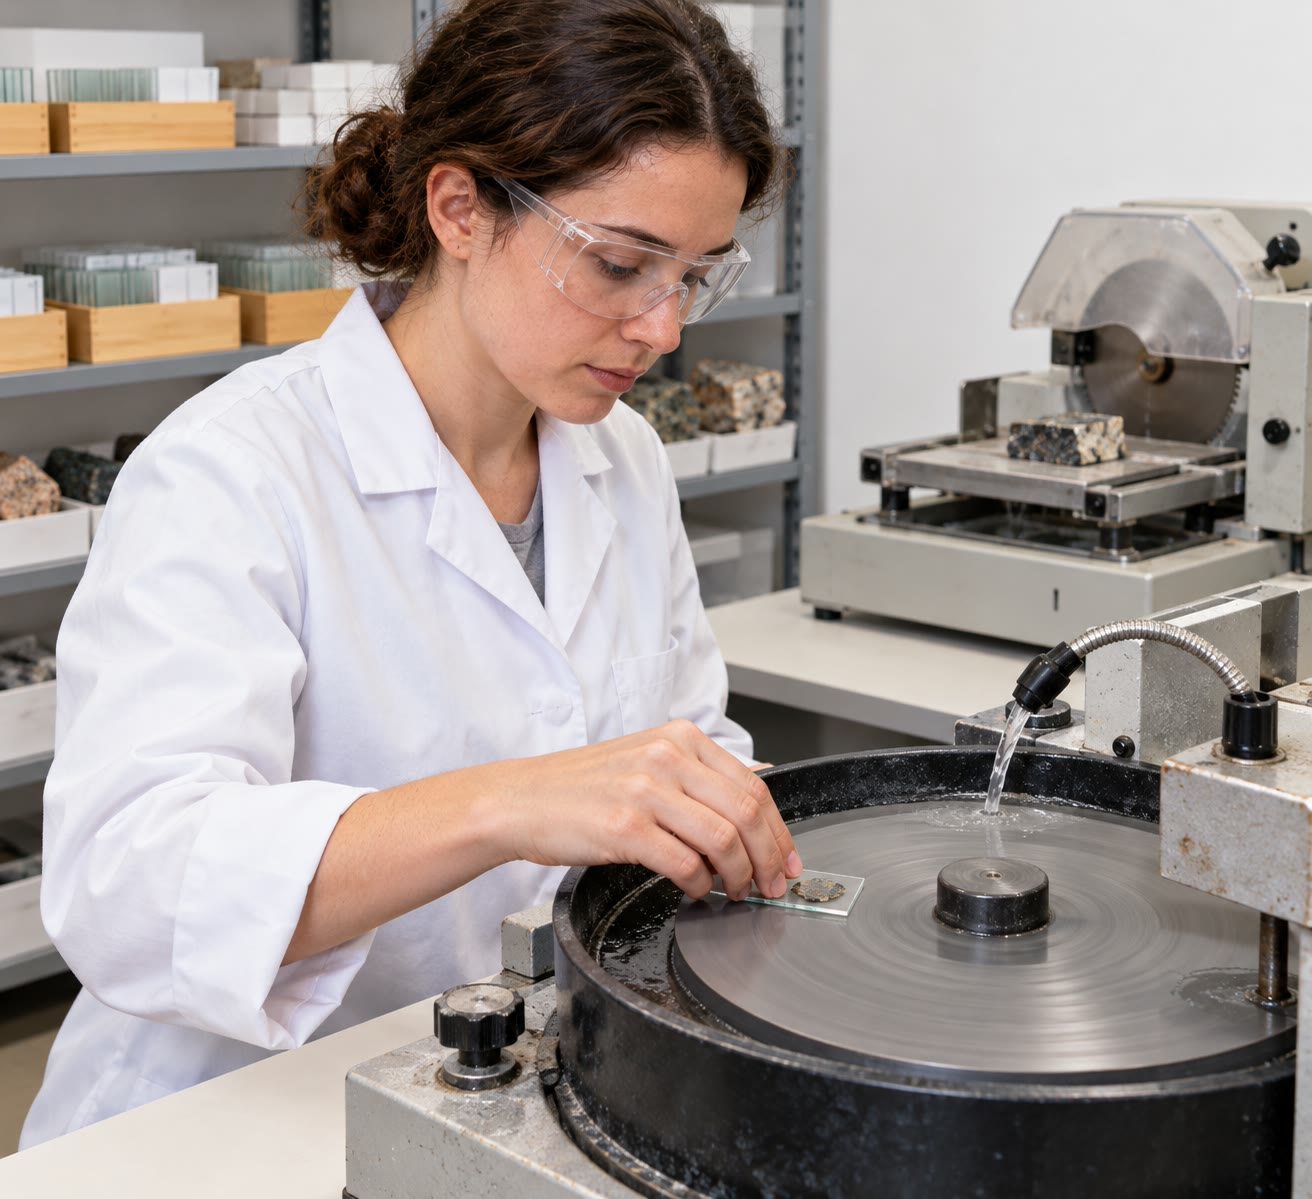
\includegraphics[width=\linewidth]{images/book3/ai/b1-thin-section-lab.jpg}
\end{minipage}
\end{inthelab}

La \omterm{def:b1:field-lab-methods-1:thin-section}{lame mince} s'étudie avec un microscope muni de deux filtres polarisants. La
polarisation rectiligne relève de la physique~: il suffit ici qu'un filtre
polarisant ne transmette que la lumière vibrant dans une direction, et que deux
filtres placés à angle droit ne transmettent rien.

\begin{definition}[Microscope polarisant, lumière polarisée non analysée, polariseurs croisés]\label{def:b1:field-lab-methods-1:microscope}
Un \emph{microscope polarisant}\index{microscope polarisant} est un microscope à
lumière transmise muni d'un filtre polarisant (le polariseur) sous une platine
qui tourne de \ang{360} devant une échelle graduée, et d'un second filtre
polarisant (l'analyseur) entre l'objectif et l'oculaire, que l'on peut introduire
dans le trajet de la lumière ou en retirer, sa direction de vibration étant à
angle droit de celle du polariseur. Avec l'analyseur retiré, le spécimen est vu
en \emph{lumière polarisée non analysée}\index{lumiere polarisee non analysee@lumière polarisée non analysée} (LPNA)~; avec l'analyseur en place, il est vu
entre \emph{polariseurs croisés}\index{polariseurs croises@polariseurs croisés} (en lumière polarisée analysée, LPA).
\end{definition}

\begin{omfigure}
\begin{tikzpicture}[font=\scriptsize, x=1cm, y=0.62cm]
\def\comp#1#2#3{\draw[fill=#3] (-1.1,#1-0.18) rectangle (1.1,#1+0.18); \node[right] at (1.3,#1) {#2};}
\draw[omThm!60, line width=3pt, -{Stealth[length=3mm]}] (0,0.3) -- (0,10.6);
\draw[fill=yellow!40] (0,0) circle (0.3); \node[right] at (1.3,0) {lampe};
\comp{1.3}{polariseur~: ne transmet qu'une direction de vibration}{omDef!25}
\draw[omDef, thick, <->] (-0.5,1.3) -- (0.5,1.3);
\draw[fill=white] (-1.0,2.3) .. controls (0,2.75) .. (1.0,2.3) .. controls (0,1.85) .. (-1.0,2.3);
\node[right] at (1.3,2.3) {condenseur};
\draw[fill=black!70] (-1.6,3.4) rectangle (1.6,3.55);
\draw[fill=icsJurassic!40] (-0.5,3.55) rectangle (0.5,3.65);
\node[right] at (1.7,3.48) {platine tournante graduée en degrés, portant la lame mince};
\draw[fill=white] (-0.45,4.5) rectangle (0.45,5.4); \node[right] at (1.3,4.95) {objectif};
\comp{6.2}{emplacement pour accessoires}{black!10}
\comp{7.2}{analyseur~: en place (polariseurs croisés) ou retiré (lumière non analysée)}{omDef!25}
\draw[omDef, thick, <->] (0,6.85) -- (0,7.55);
\comp{8.2}{lentille de Bertrand (facultative)}{black!5}
\draw[fill=white] (-0.35,9.1) rectangle (0.35,10.0); \node[right] at (1.3,9.55) {oculaire à réticule};
\end{tikzpicture}

{\small Le trajet de la lumière dans un \omterm{def:b1:field-lab-methods-1:microscope}{microscope polarisant} (schématique, de
bas en haut). Le polariseur et l'analyseur vibrent à angle droit (doubles
flèches)~; sans rien entre eux, des \omterm{def:b1:field-lab-methods-1:microscope}{polariseurs croisés} donnent un champ noir.}
\end{omfigure}

Entre \omterm{def:b1:field-lab-methods-1:microscope}{polariseurs croisés}, le verre de la lame, l'époxy et tout minéral isotrope
(dont les propriétés optiques sont les mêmes dans toutes les directions, comme
dans les cristaux cubiques) restent noirs quelle que soit la rotation de la
platine. La plupart des minéraux ne sont pas isotropes~: ils modifient la
polarisation de la lumière qui les traverse, et apparaissent en teintes de
polarisation qui changent quand la platine tourne et s'éteignent quatre fois par
tour complet. Pourquoi il en est ainsi, et comment les couleurs et les angles
identifient un minéral, fait l'objet du \cref{ch:b1:optical-mineralogy}. Les
minéraux en \omterm{def:b1:field-lab-methods-1:thin-section}{lame mince} s'examinent généralement à des grossissements d'environ
$16\times$ à $400\times$.
% ledger: jaic:magnification

\begin{omfigure}
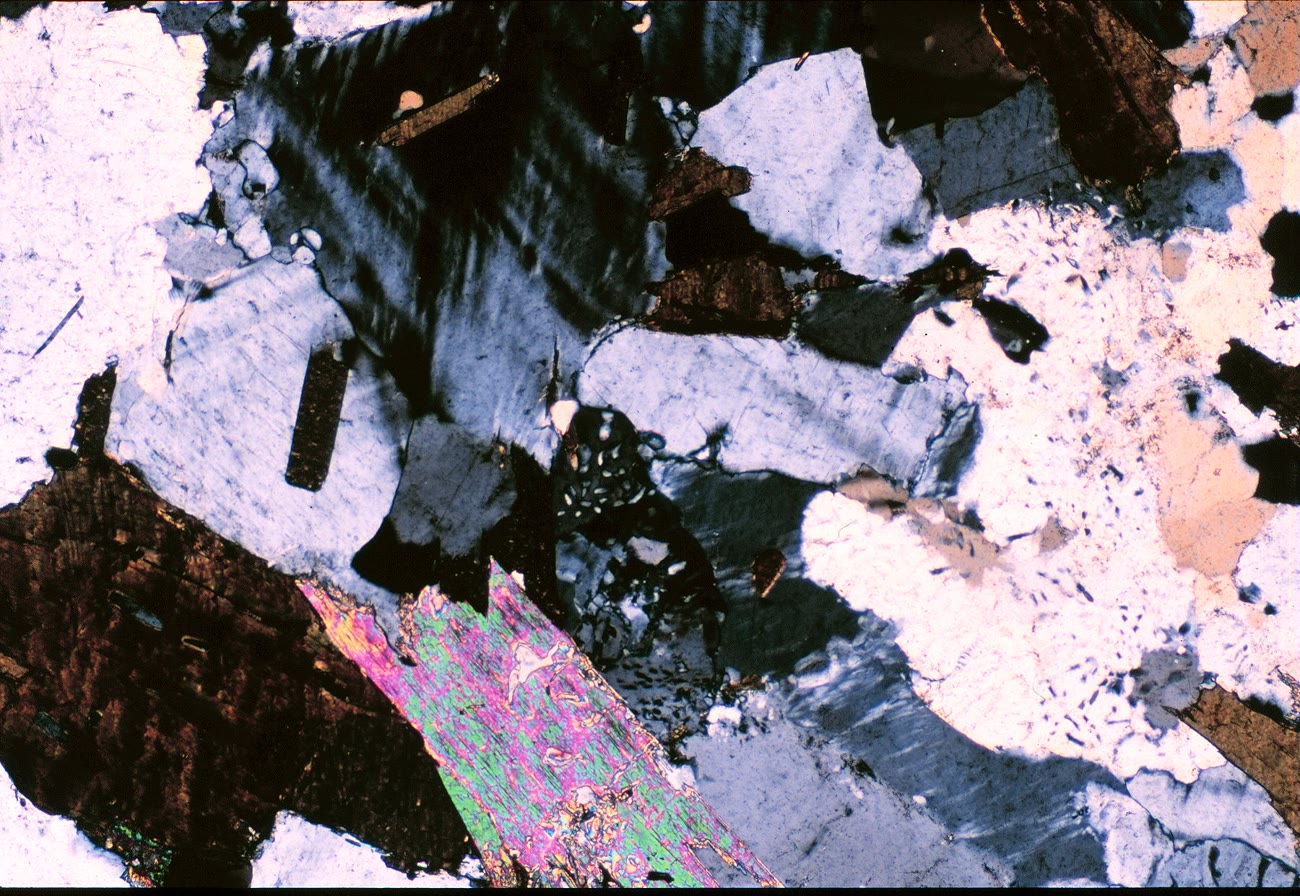
\includegraphics[width=0.55\linewidth]{images/book3/b1-granite-thin-section-xpl.jpg}
% ledger: commons:granite-xpl

{\small Un granite en \omterm{def:b1:field-lab-methods-1:thin-section}{lame mince} entre \omterm{def:b1:field-lab-methods-1:microscope}{polariseurs croisés}. La biotite est
brune, la muscovite montre des teintes de polarisation rose vif et vertes, le
plagioclase est strié par ses macles, et le quartz est blanc à gris. Photographie
Darla Sondrol, CC0 (Wikimedia Commons).}
\end{omfigure}

\begin{safety}
Le travail de terrain et de laboratoire est rendu sûr par des règles
professionnelles, non par la chance. Sur le terrain, les géologues travaillent
par deux ou laissent un plan écrit de leur itinéraire et de leur heure de
retour~; ils emportent des prévisions météorologiques, des cartes et une trousse
de secours, restent à l'écart du pied et du bord des falaises et des fronts de
carrière, et portent un casque et une protection des yeux partout où la roche
peut tomber ou éclater~; le travail sur des sites en activité suit les règles de
l'exploitant. Au laboratoire, les scies et les plateaux fonctionnent derrière des
protections, avec de l'eau pour abattre la poussière, les résines et les acides
se manipulent avec des gants et des lunettes sous aspiration, et chaque produit
chimique a sa fiche de données de sécurité. Aucune de ces activités n'est
destinée à un lecteur de ce livre agissant seul~: le chapitre décrit une pratique
professionnelle.
\end{safety}

\section{Exercices}

\begin{exercise}[$\star$]\label{exo:b1:field-lab-methods-1:1}
Un récepteur satellitaire donne des positions à environ \qty{4.9}{m} près.
Quelle taille cela représente-t-il sur une carte au 1:10\,000~? Au 1:25\,000~?
\end{exercise}

\begin{exercise}[$\star$]\label{exo:b1:field-lab-methods-1:2}
Une boussole sans réglage de déclinaison indique le \omterm{def:b1:geological-maps:attitude}{sens du pendage} \ang{052} sur
une couche. Donner le \omterm{def:b1:geological-maps:attitude}{sens du pendage} géographique si la lecture a été faite à
Reykjavik le 1\textsuperscript{er} janvier 2026, puis à Wellington le même jour
(encadré des chiffres de 2026).
\end{exercise}

\begin{exercise}[$\star$]\label{exo:b1:field-lab-methods-1:3}
Un axe de \omterm{def:b1:geological-maps:fold}{pli} plonge de \ang{20} vers \ang{015}. Écrire son orientation comme
dans le texte et donner son vecteur unitaire descendant en composantes est, nord
et haut.
\end{exercise}

\begin{exercise}[$\star$]\label{exo:b1:field-lab-methods-1:4}
Trois lectures d'un joint vertical donnent pour \omterm{def:b1:spherical-astronomy:horizontal}{azimuts} de sa normale \ang{350},
\ang{358} et \ang{006}. Calculer leur moyenne arithmétique, puis l'\omterm{def:b1:spherical-astronomy:horizontal}{azimut} de la
somme des trois vecteurs unitaires horizontaux. Quelle moyenne est la bonne~?
\end{exercise}

\begin{exercise}[$\star\star$]\label{exo:b1:field-lab-methods-1:5}
Cinq lectures du \omterm{def:b1:geological-maps:attitude}{pendage} d'une couche sont \ang{34}, \ang{37}, \ang{35},
\ang{33} et \ang{36}. Calculer leur moyenne, leur écart type et l'erreur type de
la moyenne.
\end{exercise}

\begin{exercise}[$\star\star$]\label{exo:b1:field-lab-methods-1:6}
Un géologue moyenne une lecture sur chaque flanc d'un \omterm{def:b1:geological-maps:fold}{pli} symétrique~: $090/30$
et $270/30$. Calculer la moyenne vectorielle et $\bar R$. Qu'est-ce qui n'a pas
fonctionné~?
\end{exercise}

\begin{exercise}[$\star\star$]\label{exo:b1:field-lab-methods-1:7}
Des stries sur une surface de stratification d'\omterm{def:b1:geological-maps:attitude}{attitude} $080/12$ ont pour
direction \ang{120}. Quel est leur \omterm{def:b1:field-lab-methods-1:trend-plunge}{plongement}~? Quel serait-il pour la direction
\ang{170}~?
\end{exercise}

\begin{exercise}[$\star\star$]\label{exo:b1:field-lab-methods-1:8}
À Édimbourg, la déclinaison magnétique est de \ang{-0.47} le
1\textsuperscript{er} janvier 2026 et varie de \ang{+0.20} par an. En supposant
que la variation reste régulière, quand atteint-elle zéro, et quelle est-elle le
1\textsuperscript{er} janvier 2030~?
\end{exercise}

\begin{exercise}[$\star\star$]\label{exo:b1:field-lab-methods-1:9}
Trois lectures d'une couche sont $080/10$, $080/12$ et $080/14$. Montrer que leur
moyenne vectorielle est $080/12$, calculer $\bar R$ et l'estimation
$\sqrt{2(1 - \bar R)}$ de $\theta_{\text{rms}}$, et comparer avec l'angle
quadratique moyen exact.
\end{exercise}

\begin{exercise}[$\star\star\star$]\label{exo:b1:field-lab-methods-1:10}
Une \omterm{def:b1:field-lab-methods-1:thin-section}{lame mince} coupe un grain sphérique de rayon $r$ à une distance $h$ de son
centre, $h$ étant équiprobable entre 0 et $r$. Montrer que le rayon moyen du
cercle vu dans la coupe est $\pi r/4$. Des grains de quartz de \qty{0.50}{mm} de
diamètre apparaissent en moyenne de quelle taille en \omterm{def:b1:field-lab-methods-1:thin-section}{lame mince}~?
\end{exercise}

\begin{exercise}[$\star\star\star$]\label{exo:b1:field-lab-methods-1:11}
Montrer que si chaque \omterm{def:b1:geological-maps:attitude}{sens du pendage} d'un ensemble de lectures est augmenté du
même angle $D$, le \omterm{def:b1:geological-maps:attitude}{sens du pendage} de leur moyenne vectorielle augmente de $D$ et
son \omterm{def:b1:geological-maps:attitude}{pendage} ne change pas. Pourquoi cela importe-t-il pour la correction de
déclinaison~?
\end{exercise}

\begin{exercise}[$\star\star\star$]\label{exo:b1:field-lab-methods-1:12}
Sur une couche de \omterm{def:b1:geological-maps:attitude}{pendage} \ang{12}, la normale d'une lecture isolée se disperse
avec un écart type de \ang{2} dans chacune de deux directions perpendiculaires~:
le long de la ligne de plus grande pente, ce qui change le \omterm{def:b1:geological-maps:attitude}{pendage}, et en
travers, ce qui change le \omterm{def:b1:geological-maps:attitude}{sens du pendage}. Combien de lectures faut-il pour une
erreur type de \ang{0.5} sur le \omterm{def:b1:geological-maps:attitude}{pendage} moyen~? De \ang{1} sur le \omterm{def:b1:geological-maps:attitude}{sens du pendage}
moyen~?
\end{exercise}

\section{Problème~: Une saison de terrain sur le flanc est de Varden}

\begin{problem}[{Problème du week-end --- moyenner douze lectures de boussole, mesurer
leur dispersion, les corriger et les comparer aux sondages}]
\label{pb:b1:field-lab-methods-1:1}
% readings: figdata/bachelor-1/attitude_stats.py (part normals); values: calc/ch06.py
Un géologue a mesuré la stratification du flanc est de l'\omterm{def:b1:geological-maps:fold}{anticlinal} de Varden en
douze stations, avec une boussole réglée pour la déclinaison, en arrondissant au
degré. Le tableau donne chaque lecture (\omterm{def:b1:geological-maps:attitude}{sens du pendage}/\omterm{def:b1:geological-maps:attitude}{pendage}) et les
composantes de sa normale unitaire dirigée vers le haut
$\vec n = (n_E, n_N, n_U)$, arrondies à quatre décimales.
\begin{center}
\small
\begin{tabular}{rcccc@{\qquad}rcccc}
\hline
 & lecture & $n_E$ & $n_N$ & $n_U$ & & lecture & $n_E$ & $n_N$ & $n_U$ \\
\hline
1 & $076/11$ & 0.1851 & 0.0462 & 0.9816 & 7 & $083/11$ & 0.1894 & 0.0233 & 0.9816 \\
2 & $081/13$ & 0.2222 & 0.0352 & 0.9744 & 8 & $083/12$ & 0.2064 & 0.0253 & 0.9781 \\
3 & $078/16$ & 0.2696 & 0.0573 & 0.9613 & 9 & $085/12$ & 0.2071 & 0.0181 & 0.9781 \\
4 & $081/11$ & 0.1885 & 0.0298 & 0.9816 & 10 & $078/11$ & 0.1866 & 0.0397 & 0.9816 \\
5 & $076/10$ & 0.1685 & 0.0420 & 0.9848 & 11 & $081/13$ & & & \\
6 & $083/14$ & 0.2401 & 0.0295 & 0.9703 & 12 & $082/11$ & & & \\
\hline
\end{tabular}
\end{center}

\medskip
\noindent\textbf{Partie I --- L'attitude moyenne.}
\begin{enumerate}
  \item Calculer les moyennes arithmétiques des douze \omterm{def:b1:geological-maps:attitude}{sens du pendage} et des
        douze \omterm{def:b1:geological-maps:attitude}{pendages}.
  \item Donner un exemple de deux lectures pour lesquelles la moyenne
        arithmétique des \omterm{def:b1:geological-maps:attitude}{sens du pendage} est absurde, et dire pourquoi elle est
        sans danger ici.
  \item Montrer que $\vec n = (\sin\delta\sin\alpha, \sin\delta\cos\alpha,
        \cos\delta)$ est un vecteur unitaire perpendiculaire à la ligne de
        \omterm{def:b1:geological-maps:attitude}{pendage} et à la ligne de direction du plan $\alpha/\delta$.
  \item Compléter le tableau pour les lectures 11 et 12.
  \item Calculer la résultante $\vec S$ des douze normales.
  \item Calculer $\|\vec S\|$ et la longueur résultante moyenne $\bar R$.
  \item En déduire la moyenne vectorielle~: son \omterm{def:b1:geological-maps:attitude}{sens du pendage} et son \omterm{def:b1:geological-maps:attitude}{pendage}.
\end{enumerate}

\medskip
\noindent\textbf{Partie II --- La dispersion.}
\begin{enumerate}[resume]
  \item Calculer les écarts types empiriques des \omterm{def:b1:geological-maps:attitude}{sens du pendage} et des
        \omterm{def:b1:geological-maps:attitude}{pendages}.
  \item À l'aide de la \cref{prop:b1:field-lab-methods-1:vector-mean}, estimer
        l'angle quadratique moyen $\theta_{\text{rms}}$ entre les lectures et
        leur moyenne, en degrés.
  \item Prévoir $\theta_{\text{rms}}$ à partir des deux écarts types de la
        question 8 et de la formule d'erreur du chapitre, et comparer.
  \item Lequel des deux écarts types contribue le plus à
        $\theta_{\text{rms}}$, et pourquoi~?
  \item Calculer les erreurs types du \omterm{def:b1:geological-maps:attitude}{pendage} moyen et du \omterm{def:b1:geological-maps:attitude}{sens du pendage}
        moyen.
  \item La dispersion des \omterm{def:b1:geological-maps:attitude}{sens du pendage}, \ang{2.9}, est-elle le signe d'une
        mesure négligente~? Expliquer.
\end{enumerate}

\medskip
\noindent\textbf{Partie III --- La déclinaison.}
\begin{enumerate}[resume]
  \item Une seconde géologue a oublié de régler la déclinaison. Ses douze
        lectures ont pour moyenne vectorielle $083.1/12.1$ en \omterm{def:b1:spherical-astronomy:horizontal}{azimuts}
        magnétiques. Supposons que la déclinaison magnétique dans les collines
        de Varden cette année-là soit de \ang{2.5} ouest. Quelle est sa moyenne
        en \omterm{def:b1:spherical-astronomy:horizontal}{azimuts} géographiques~?
  \item Pourquoi son \omterm{def:b1:geological-maps:attitude}{pendage} moyen est-il juste sans correction~?
  \item Aurait-elle pu corriger chaque lecture avant de moyenner, plutôt que la
        moyenne~? Cela change-t-il la réponse
        (\cref{exo:b1:field-lab-methods-1:11})~?
  \item Dix ans plus tard, un étudiant réutilise son réglage de déclinaison alors
        que la déclinaison a varié de \ang{0.2} par an. Quelle est l'erreur,
        comparée à l'erreur type de la question 12~?
  \item Donner la direction de l'\omterm{def:b1:geological-maps:attitude}{attitude} moyenne de la première géologue par la
        règle de la main droite.
\end{enumerate}

\medskip
\noindent\textbf{Partie IV --- Boussole et sondages.}
\begin{enumerate}[resume]
  \item À partir de trois sondages, le \cref{ch:b1:geological-maps} a trouvé
        l'\omterm{def:b1:geological-maps:attitude}{attitude} $080.6/12.2$ pour la base du calcaire. La comparer à la
        moyenne vectorielle de la question 7, angle par angle.
  \item Calculer l'angle entre les deux normales.
  \item L'erreur type de la direction moyenne est d'environ
        $\theta_{\text{rms}}/\sqrt N$. La différence de la question 20 est-elle
        significative~?
  \item Combien de lectures faudrait-il pour diviser cette erreur type par
        deux~?
  \item Citer deux erreurs qu'aucun nombre de lectures ne réduirait.
  \item Donner l'\omterm{def:b1:geological-maps:attitude}{attitude} moyenne du flanc est d'après les douze lectures, sous
        la forme \omterm{def:b1:geological-maps:attitude}{sens du pendage}/\omterm{def:b1:geological-maps:attitude}{pendage} arrondis au degré.
\end{enumerate}
\end{problem}
